% Source: fourier_course.tex
\begin{notechapter}
% ---- chapter-local definitions ----
\forgetcs\sinc\newcommand{\sinc}{\operatorname{sinc}}
\forgetcs\rect\newcommand{\rect}{\operatorname{rect}}
\forgetcs\R\newcommand{\R}{\mathbb{R}}
\forgetcs\C\newcommand{\C}{\mathbb{C}}
\forgetcs\Z\newcommand{\Z}{\mathbb{Z}}
\forgetcs\N\newcommand{\N}{\mathbb{N}}
\forgetcs\fourier\newcommand{\fourier}{\mathcal{F}}
\forgetcs\abs\newcommand{\abs}[1]{\left|#1\right|}
\forgetcs\norm\newcommand{\norm}[1]{\left\|#1\right\|}
\forgetcs\inner\newcommand{\inner}[2]{\left\langle #1, #2 \right\rangle}
% -----------------------------------
\chapter{Fourier Analysis}\label{ch:fourier-analysis}
\chaptersubtitle{From series to fast transforms}

\begin{abstract}
This document provides a mathematically rigorous treatment of the Fourier family of transforms: Fourier series, Fourier transform, Discrete-Time Fourier Transform (DTFT), Discrete Fourier Transform (DFT), and Fast Fourier Transform (FFT). We carefully establish the conditions under which each method applies, prove key theorems, and demonstrate the relationships between these techniques. The presentation assumes familiarity with real analysis, complex analysis, and linear algebra at the advanced undergraduate level.
\end{abstract}

\section{Introduction and Motivation}

The Fourier family of techniques allows us to represent signals as superpositions of sinusoids. The choice of which technique to use depends on the nature of the signal:

\begin{itemize}
\item Is the signal continuous or discrete in time?
\item Is the signal periodic or aperiodic?
\item Is the signal of finite or infinite duration?
\item Do we have practical computational constraints?
\end{itemize}

\begin{center}
\begin{tabular}{|l|c|c|c|}
\hline
\textbf{Method} & \textbf{Time Domain} & \textbf{Periodicity} & \textbf{Frequency Domain} \\
\hline
Fourier Series & Continuous, Periodic & Periodic & Discrete \\
Fourier Transform & Continuous, Aperiodic & Aperiodic & Continuous \\
DTFT & Discrete, Aperiodic & Aperiodic & Continuous, Periodic \\
DFT & Discrete, Periodic & Periodic & Discrete, Periodic \\
\hline
\end{tabular}
\end{center}

\section{Mathematical Preliminaries}

\subsection{Function Spaces}

\begin{definition}[$L^1$ Space]
The space $L^1(\R)$ consists of all Lebesgue measurable functions $f:\R \to \C$ such that
\[
\norm{f}_1 = \int_{-\infty}^{\infty} \abs{f(t)} \, dt < \infty.
\]
\end{definition}

\begin{definition}[$L^2$ Space]
The space $L^2(\R)$ consists of all Lebesgue measurable functions $f:\R \to \C$ such that
\[
\norm{f}_2 = \sqrt{\int_{-\infty}^{\infty} \abs{f(t)}^2 \, dt} < \infty.
\]
This is a Hilbert space with inner product
\[
\inner{f}{g} = \int_{-\infty}^{\infty} f(t) \overline{g(t)} \, dt.
\]
\end{definition}

\begin{theorem}[Hölder's Inequality]
If $p, q \geq 1$ satisfy $\frac{1}{p} + \frac{1}{q} = 1$, then for $f \in L^p$ and $g \in L^q$,
\[
\int_{-\infty}^{\infty} \abs{f(t)g(t)} \, dt \leq \norm{f}_p \norm{g}_q.
\]
\end{theorem}

\begin{corollary}
$L^1(\R) \cap L^2(\R) \subset L^1(\R)$ and $L^2(\R) \subset L^1_{\text{loc}}(\R)$.
\end{corollary}

\subsection{Periodic Functions}

\begin{definition}[Periodic Function]
A function $f:\R \to \C$ is \emph{$T$-periodic} if $f(t+T) = f(t)$ for all $t \in \R$.
\end{definition}

For periodic functions, we define:
\[
L^2([0,T]) = \left\{ f:[0,T] \to \C : \int_0^T \abs{f(t)}^2 \, dt < \infty \right\}.
\]

\section{Fourier Series}

\subsection{Motivation and Setting}

Consider a $T$-periodic function $f:\R \to \C$. Since the function repeats every $T$ seconds, it is natural to ask whether we can represent it as a sum of harmonically related sinusoids.

\begin{definition}[Fourier Series]
Let $f$ be a $T$-periodic function in $L^2([0,T])$. The \emph{Fourier series} of $f$ is
\[
f(t) \sim \sum_{n=-\infty}^{\infty} c_n e^{i 2\pi n t/T},
\]
where the \emph{Fourier coefficients} are given by
\[
c_n = \frac{1}{T} \int_0^T f(t) e^{-i 2\pi n t/T} \, dt.
\]
\end{definition}

\begin{remark}
We use the symbol $\sim$ to denote that the series is associated with $f$. Convergence requires further conditions.
\end{remark}

\subsection{Orthogonality of Complex Exponentials}

The key insight is that the complex exponentials form an orthogonal basis.

\begin{lemma}[Orthogonality]
For $m, n \in \Z$,
\[
\frac{1}{T}\int_0^T e^{i 2\pi n t/T} e^{-i 2\pi m t/T} \, dt = \delta_{mn} = \begin{cases}
1 & \text{if } m = n \\
0 & \text{if } m \neq n.
\end{cases}
\]
\end{lemma}

\begin{proof}
\[
\frac{1}{T}\int_0^T e^{i 2\pi (n-m) t/T} \, dt = \frac{1}{T} \left[ \frac{T}{i 2\pi (n-m)} e^{i 2\pi (n-m) t/T} \right]_0^T
\]
If $n \neq m$:
\[
= \frac{1}{i 2\pi (n-m)} \left( e^{i 2\pi (n-m)} - 1 \right) = \frac{1}{i 2\pi (n-m)} (1 - 1) = 0.
\]
If $n = m$:
\[
\frac{1}{T}\int_0^T e^{0} \, dt = \frac{1}{T} \cdot T = 1.
\]
\end{proof}

\subsection{Derivation of Fourier Coefficients}

To find the coefficients $c_n$, we use the orthogonality relation. Multiply both sides of the Fourier series by $e^{-i 2\pi m t/T}$ and integrate:

\begin{align*}
\int_0^T f(t) e^{-i 2\pi m t/T} \, dt &= \int_0^T \left( \sum_{n=-\infty}^{\infty} c_n e^{i 2\pi n t/T} \right) e^{-i 2\pi m t/T} \, dt \\
&= \sum_{n=-\infty}^{\infty} c_n \int_0^T e^{i 2\pi (n-m) t/T} \, dt \\
&= \sum_{n=-\infty}^{\infty} c_n \cdot T \delta_{mn} \\
&= T c_m.
\end{align*}

Therefore,
\[
c_m = \frac{1}{T} \int_0^T f(t) e^{-i 2\pi m t/T} \, dt.
\]

\subsection{Convergence Theorems}

\begin{theorem}[Dirichlet Conditions]
Let $f$ be a $T$-periodic function. If $f$ satisfies:
\begin{enumerate}
\item $f$ is absolutely integrable over one period: $\int_0^T \abs{f(t)} \, dt < \infty$,
\item $f$ has a finite number of maxima and minima in one period,
\item $f$ has a finite number of discontinuities in one period,
\end{enumerate}
then the Fourier series of $f$ converges pointwise to
\[
\frac{f(t^+) + f(t^-)}{2}
\]
at every point $t$, where $f(t^+)$ and $f(t^-)$ denote the right and left limits.
\end{theorem}

\begin{theorem}[Mean Square Convergence]
If $f \in L^2([0,T])$, then
\[
\lim_{N \to \infty} \int_0^T \left| f(t) - \sum_{n=-N}^{N} c_n e^{i 2\pi n t/T} \right|^2 dt = 0.
\]
\end{theorem}

\begin{theorem}[Parseval's Identity for Fourier Series]
For $f \in L^2([0,T])$,
\[
\frac{1}{T} \int_0^T \abs{f(t)}^2 \, dt = \sum_{n=-\infty}^{\infty} \abs{c_n}^2.
\]
\end{theorem}

\begin{proof}
Using the inner product structure:
\begin{align*}
\frac{1}{T} \int_0^T \abs{f(t)}^2 \, dt &= \frac{1}{T} \int_0^T f(t) \overline{f(t)} \, dt \\
&= \frac{1}{T} \int_0^T f(t) \overline{\sum_{m} c_m e^{i 2\pi m t/T}} \, dt \\
&= \frac{1}{T} \int_0^T f(t) \sum_{m} \overline{c_m} e^{-i 2\pi m t/T} \, dt \\
&= \sum_{m} \overline{c_m} \frac{1}{T} \int_0^T f(t) e^{-i 2\pi m t/T} \, dt \\
&= \sum_{m} \overline{c_m} c_m = \sum_{m} \abs{c_m}^2.
\end{align*}
\end{proof}

\subsection{Real Fourier Series}

For real-valued functions, we often use the trigonometric form.

\begin{proposition}
If $f:\R \to \R$ is real and $T$-periodic, then $c_{-n} = \overline{c_n}$, and
\[
f(t) = a_0 + \sum_{n=1}^{\infty} \left( a_n \cos\frac{2\pi n t}{T} + b_n \sin\frac{2\pi n t}{T} \right),
\]
where
\begin{align*}
a_0 &= c_0 = \frac{1}{T} \int_0^T f(t) \, dt, \\
a_n &= 2\text{Re}(c_n) = \frac{2}{T} \int_0^T f(t) \cos\frac{2\pi n t}{T} \, dt, \\
b_n &= -2\text{Im}(c_n) = \frac{2}{T} \int_0^T f(t) \sin\frac{2\pi n t}{T} \, dt.
\end{align*}
\end{proposition}

\begin{proof}
Since $c_n e^{i 2\pi n t/T} + c_{-n} e^{-i 2\pi n t/T} = c_n e^{i 2\pi n t/T} + \overline{c_n} e^{-i 2\pi n t/T}$, we have
\begin{align*}
&= (a_n - ib_n)(e^{i 2\pi n t/T}) + (a_n + ib_n)(e^{-i 2\pi n t/T}) \\
&= a_n(e^{i 2\pi n t/T} + e^{-i 2\pi n t/T}) - ib_n(e^{i 2\pi n t/T} - e^{-i 2\pi n t/T}) \\
&= 2a_n \cos\frac{2\pi n t}{T} + 2b_n \sin\frac{2\pi n t}{T}.
\end{align*}
\end{proof}

\subsection{Example: Square Wave}

\begin{example}
Consider the square wave with period $T = 2\pi$:
\[
f(t) = \begin{cases}
1 & \text{if } 0 < t < \pi \\
-1 & \text{if } \pi < t < 2\pi
\end{cases}
\]
extended periodically.

The Fourier coefficients are:
\begin{align*}
c_n &= \frac{1}{2\pi} \int_0^{2\pi} f(t) e^{-int} \, dt \\
&= \frac{1}{2\pi} \left( \int_0^{\pi} e^{-int} \, dt - \int_{\pi}^{2\pi} e^{-int} \, dt \right) \\
&= \frac{1}{2\pi} \left[ \frac{e^{-int}}{-in} \right]_0^{\pi} - \frac{1}{2\pi} \left[ \frac{e^{-int}}{-in} \right]_{\pi}^{2\pi} \\
&= \frac{1}{-i 2\pi n} \left( e^{-in\pi} - 1 - e^{-i 2\pi n} + e^{-in\pi} \right) \\
&= \frac{1}{-i 2\pi n} \left( 2e^{-in\pi} - 1 - 1 \right) \\
&= \frac{1}{-i 2\pi n} \left( 2\cos(n\pi) - 2i\sin(n\pi) - 2 \right) \\
&= \frac{1}{-i 2\pi n} \left( 2(-1)^n - 2 \right) \\
&= \frac{(-1)^n - 1}{-i\pi n}.
\end{align*}

For $n$ even: $c_n = 0$.
For $n$ odd: $c_n = \frac{-2}{-i\pi n} = \frac{2i}{\pi n}$.

Thus,
\[
f(t) = \sum_{\substack{n \text{ odd} \\ n \neq 0}} \frac{2i}{\pi n} e^{int} = \frac{4}{\pi} \sum_{k=0}^{\infty} \frac{\sin((2k+1)t)}{2k+1}.
\]
\end{example}

\section{Fourier Transform}

\subsection{Motivation: From Periodic to Aperiodic}

The Fourier transform extends the idea of Fourier series to aperiodic functions by taking the limit as the period $T \to \infty$.

Consider a function $f \in L^1(\R)$. We can create a periodic function $f_T$ that equals $f$ on $[-T/2, T/2]$ and is extended periodically. As $T \to \infty$, $f_T \to f$.

The Fourier series of $f_T$ is:
\[
f_T(t) = \sum_{n=-\infty}^{\infty} c_n e^{i 2\pi n t/T}, \quad c_n = \frac{1}{T} \int_{-T/2}^{T/2} f_T(t) e^{-i 2\pi n t/T} \, dt.
\]

Define $\omega_n = 2\pi n/T$ and $\Delta \omega = 2\pi/T$. Then:
\[
c_n = \frac{1}{T} \int_{-T/2}^{T/2} f(t) e^{-i\omega_n t} \, dt = \frac{\Delta \omega}{2\pi} \int_{-T/2}^{T/2} f(t) e^{-i\omega_n t} \, dt.
\]

As $T \to \infty$, $\Delta \omega \to d\omega$ and the sum becomes an integral.

\subsection{Definition and Basic Properties}

\begin{definition}[Fourier Transform]
For $f \in L^1(\R)$, the \emph{Fourier transform} is
\[
\hat{f}(\omega) = \fourier\{f\}(\omega) = \int_{-\infty}^{\infty} f(t) e^{-i\omega t} \, dt.
\]
The \emph{inverse Fourier transform} is
\[
f(t) = \fourier^{-1}\{\hat{f}\}(t) = \frac{1}{2\pi} \int_{-\infty}^{\infty} \hat{f}(\omega) e^{i\omega t} \, d\omega.
\]
\end{definition}

\begin{remark}
There are several conventions for the Fourier transform differing in the placement of factors of $2\pi$ and the sign of the exponent. We use the angular frequency convention where $\omega = 2\pi f$.
\end{remark}

\begin{theorem}[Riemann-Lebesgue Lemma]
If $f \in L^1(\R)$, then $\hat{f}$ is continuous and
\[
\lim_{\abs{\omega} \to \infty} \hat{f}(\omega) = 0.
\]
\end{theorem}

\begin{proof}
Continuity follows from the dominated convergence theorem. For the decay, use integration by parts or the fact that oscillatory integrals average to zero.
\end{proof}

\subsection{Inversion Formula}

\begin{theorem}[Fourier Inversion Theorem]
Let $f \in L^1(\R)$ with $\hat{f} \in L^1(\R)$. If $f$ is continuous at $t$, then
\[
f(t) = \frac{1}{2\pi} \int_{-\infty}^{\infty} \hat{f}(\omega) e^{i\omega t} \, d\omega.
\]
If $f$ has a jump discontinuity at $t$, the right side equals $(f(t^+) + f(t^-))/2$.
\end{theorem}

\subsection{Plancherel Theorem and $L^2$ Theory}

\begin{theorem}[Plancherel Theorem]
The Fourier transform extends to an isometry on $L^2(\R)$:
\[
\int_{-\infty}^{\infty} \abs{f(t)}^2 \, dt = \frac{1}{2\pi} \int_{-\infty}^{\infty} \abs{\hat{f}(\omega)}^2 \, d\omega.
\]
\end{theorem}

\begin{corollary}[Parseval's Identity]
For $f, g \in L^2(\R)$,
\[
\int_{-\infty}^{\infty} f(t) \overline{g(t)} \, dt = \frac{1}{2\pi} \int_{-\infty}^{\infty} \hat{f}(\omega) \overline{\hat{g}(\omega)} \, d\omega.
\]
\end{corollary}

\subsection{Properties of the Fourier Transform}

\begin{proposition}[Linearity]
For $\alpha, \beta \in \C$ and $f, g \in L^1(\R)$,
\[
\fourier\{\alpha f + \beta g\} = \alpha \hat{f} + \beta \hat{g}.
\]
\end{proposition}

\begin{proposition}[Time Shift]
\[
\fourier\{f(t - t_0)\}(\omega) = e^{-i\omega t_0} \hat{f}(\omega).
\]
\end{proposition}

\begin{proof}
\begin{align*}
\fourier\{f(t - t_0)\}(\omega) &= \int_{-\infty}^{\infty} f(t - t_0) e^{-i\omega t} \, dt \\
&= \int_{-\infty}^{\infty} f(u) e^{-i\omega (u + t_0)} \, du \quad (u = t - t_0) \\
&= e^{-i\omega t_0} \int_{-\infty}^{\infty} f(u) e^{-i\omega u} \, du \\
&= e^{-i\omega t_0} \hat{f}(\omega).
\end{align*}
\end{proof}

\begin{proposition}[Frequency Shift / Modulation]
\[
\fourier\{e^{i\omega_0 t} f(t)\}(\omega) = \hat{f}(\omega - \omega_0).
\]
\end{proposition}

\begin{proposition}[Scaling]
For $a \neq 0$,
\[
\fourier\{f(at)\}(\omega) = \frac{1}{\abs{a}} \hat{f}\left(\frac{\omega}{a}\right).
\]
\end{proposition}

\begin{proof}
For $a > 0$:
\begin{align*}
\fourier\{f(at)\}(\omega) &= \int_{-\infty}^{\infty} f(at) e^{-i\omega t} \, dt \\
&= \int_{-\infty}^{\infty} f(u) e^{-i\omega u/a} \frac{du}{a} \quad (u = at) \\
&= \frac{1}{a} \hat{f}\left(\frac{\omega}{a}\right).
\end{align*}
For $a < 0$, the limits reverse and we get a factor of $1/\abs{a}$.
\end{proof}

\begin{proposition}[Differentiation in Time]
If $f$ and $f'$ are in $L^1(\R)$ and $\lim_{\abs{t} \to \infty} f(t) = 0$, then
\[
\fourier\{f'(t)\}(\omega) = i\omega \hat{f}(\omega).
\]
\end{proposition}

\begin{proof}
Using integration by parts:
\begin{align*}
\fourier\{f'(t)\}(\omega) &= \int_{-\infty}^{\infty} f'(t) e^{-i\omega t} \, dt \\
&= \left[ f(t) e^{-i\omega t} \right]_{-\infty}^{\infty} - \int_{-\infty}^{\infty} f(t) (-i\omega) e^{-i\omega t} \, dt \\
&= 0 + i\omega \int_{-\infty}^{\infty} f(t) e^{-i\omega t} \, dt \\
&= i\omega \hat{f}(\omega).
\end{align*}
\end{proof}

\begin{proposition}[Differentiation in Frequency]
If $tf(t) \in L^1(\R)$, then $\hat{f}$ is differentiable and
\[
\frac{d\hat{f}}{d\omega}(\omega) = \fourier\{-it f(t)\}(\omega).
\]
\end{proposition}

\begin{proposition}[Convolution Theorem]
If $f, g \in L^1(\R)$, then
\[
\fourier\{f * g\} = \hat{f} \cdot \hat{g},
\]
where $(f * g)(t) = \int_{-\infty}^{\infty} f(\tau) g(t - \tau) \, d\tau$ is the convolution.
\end{proposition}

\begin{proof}
\begin{align*}
\fourier\{f * g\}(\omega) &= \int_{-\infty}^{\infty} \left( \int_{-\infty}^{\infty} f(\tau) g(t - \tau) \, d\tau \right) e^{-i\omega t} \, dt \\
&= \int_{-\infty}^{\infty} f(\tau) \left( \int_{-\infty}^{\infty} g(t - \tau) e^{-i\omega t} \, dt \right) d\tau \\
&= \int_{-\infty}^{\infty} f(\tau) e^{-i\omega \tau} \left( \int_{-\infty}^{\infty} g(u) e^{-i\omega u} \, du \right) d\tau \\
&= \hat{g}(\omega) \int_{-\infty}^{\infty} f(\tau) e^{-i\omega \tau} \, d\tau \\
&= \hat{f}(\omega) \hat{g}(\omega).
\end{align*}
\end{proof}

\subsection{Important Fourier Transform Pairs}

\begin{example}[Rectangular Pulse]
\[
\rect(t) = \begin{cases}
1 & \abs{t} < 1/2 \\
0 & \abs{t} > 1/2
\end{cases}
\]
Then
\[
\fourier\{\rect(t)\}(\omega) = \int_{-1/2}^{1/2} e^{-i\omega t} \, dt = \frac{2\sin(\omega/2)}{\omega} = \sinc(\omega/2\pi),
\]
where $\sinc(x) = \sin(\pi x)/(\pi x)$.
\end{example}

\begin{example}[Gaussian]
For $f(t) = e^{-\alpha t^2}$ with $\alpha > 0$,
\[
\hat{f}(\omega) = \sqrt{\frac{\pi}{\alpha}} e^{-\omega^2/(4\alpha)}.
\]
The Gaussian is its own Fourier transform (up to scaling).
\end{example}

\begin{proof}
Let $I(\omega) = \int_{-\infty}^{\infty} e^{-\alpha t^2 - i\omega t} \, dt$.

Complete the square:
\[
-\alpha t^2 - i\omega t = -\alpha \left( t + \frac{i\omega}{2\alpha} \right)^2 - \frac{\omega^2}{4\alpha}.
\]

Shift the contour:
\[
I(\omega) = e^{-\omega^2/(4\alpha)} \int_{-\infty}^{\infty} e^{-\alpha u^2} \, du = e^{-\omega^2/(4\alpha)} \sqrt{\frac{\pi}{\alpha}}.
\]
\end{proof}

\begin{example}[Dirac Delta]
The Dirac delta $\delta(t)$ (technically a distribution) has
\[
\hat{\delta}(\omega) = 1.
\]
Conversely,
\[
\fourier\{1\}(\omega) = 2\pi \delta(\omega).
\]
\end{example}

\section{Discrete-Time Fourier Transform (DTFT)}

\subsection{From Continuous to Discrete Time}

When we sample a continuous signal $f(t)$ at intervals $T_s$, we obtain a discrete sequence $x[n] = f(nT_s)$ for $n \in \Z$. The DTFT analyzes such sequences.

\begin{definition}[DTFT]
For a sequence $\{x[n]\}_{n=-\infty}^{\infty}$ with $\sum_{n=-\infty}^{\infty} \abs{x[n]} < \infty$, the \emph{Discrete-Time Fourier Transform} is
\[
X(e^{i\omega}) = \sum_{n=-\infty}^{\infty} x[n] e^{-i\omega n}.
\]
The inverse DTFT is
\[
x[n] = \frac{1}{2\pi} \int_{-\pi}^{\pi} X(e^{i\omega}) e^{i\omega n} \, d\omega.
\]
\end{definition}

\begin{remark}
The frequency variable $\omega$ is now normalized (dimensionless). The actual frequency is $f = \omega/(2\pi T_s)$ Hz.
\end{remark}

\subsection{Periodicity in Frequency}

\begin{proposition}
$X(e^{i\omega})$ is $2\pi$-periodic in $\omega$:
\[
X(e^{i(\omega + 2\pi)}) = X(e^{i\omega}).
\]
\end{proposition}

\begin{proof}
\[
X(e^{i(\omega + 2\pi)}) = \sum_{n=-\infty}^{\infty} x[n] e^{-i(\omega + 2\pi)n} = \sum_{n=-\infty}^{\infty} x[n] e^{-i\omega n} e^{-i 2\pi n} = \sum_{n=-\infty}^{\infty} x[n] e^{-i\omega n} = X(e^{i\omega}).
\]
\end{proof}

This periodicity reflects the \emph{aliasing} phenomenon: frequencies differing by multiples of the sampling frequency are indistinguishable.

\subsection{Sampling Theorem}

\begin{theorem}[Nyquist-Shannon Sampling Theorem]
Let $f(t)$ be a bandlimited signal with $\hat{f}(\omega) = 0$ for $\abs{\omega} > \omega_{\max}$. If $f$ is sampled at rate $\omega_s = 2\pi/T_s > 2\omega_{\max}$ (the Nyquist rate), then $f$ can be perfectly reconstructed from its samples:
\[
f(t) = \sum_{n=-\infty}^{\infty} f(nT_s) \sinc\left(\frac{t - nT_s}{T_s}\right).
\]
\end{theorem}

\subsection{Relationship to Fourier Transform}

If $x[n] = f(nT_s)$ where $f \in L^1(\R)$, then
\[
X(e^{i\omega}) = \frac{1}{T_s} \sum_{k=-\infty}^{\infty} \hat{f}\left(\frac{\omega - 2\pi k}{T_s}\right).
\]

This shows that the DTFT is a periodically replicated version of the continuous Fourier transform.

\subsection{Properties of the DTFT}

\begin{proposition}[Time Shift]
\[
\text{DTFT}\{x[n - n_0]\} = e^{-i\omega n_0} X(e^{i\omega}).
\]
\end{proposition}

\begin{proposition}[Frequency Shift]
\[
\text{DTFT}\{e^{i\omega_0 n} x[n]\} = X(e^{i(\omega - \omega_0)}).
\]
\end{proposition}

\begin{proposition}[Convolution]
For discrete convolution $(x * h)[n] = \sum_{k=-\infty}^{\infty} x[k] h[n-k]$,
\[
\text{DTFT}\{x * h\} = X(e^{i\omega}) H(e^{i\omega}).
\]
\end{proposition}

\begin{proposition}[Parseval's Identity]
\[
\sum_{n=-\infty}^{\infty} \abs{x[n]}^2 = \frac{1}{2\pi} \int_{-\pi}^{\pi} \abs{X(e^{i\omega})}^2 \, d\omega.
\]
\end{proposition}

\section{Discrete Fourier Transform (DFT)}

\subsection{Finite-Length Sequences}

In practice, we work with finite-length sequences. The DFT is the appropriate tool for this setting.

\begin{definition}[DFT]
For a finite sequence $\{x[n]\}_{n=0}^{N-1}$ of length $N$, the \emph{Discrete Fourier Transform} is
\[
X[k] = \sum_{n=0}^{N-1} x[n] e^{-i 2\pi kn/N}, \quad k = 0, 1, \ldots, N-1.
\]
The \emph{inverse DFT} (IDFT) is
\[
x[n] = \frac{1}{N} \sum_{k=0}^{N-1} X[k] e^{i 2\pi kn/N}, \quad n = 0, 1, \ldots, N-1.
\]
\end{definition}

\subsection{Matrix Formulation}

Define the \emph{DFT matrix}:
\[
W_N = e^{-i 2\pi/N}, \quad [F_N]_{kn} = W_N^{kn} = e^{-i 2\pi kn/N}.
\]

Then:
\[
\mathbf{X} = F_N \mathbf{x}, \quad \mathbf{x} = \frac{1}{N} F_N^* \mathbf{X},
\]
where $F_N^*$ is the conjugate transpose.

\begin{lemma}
$F_N$ is unitary up to scaling: $F_N^* F_N = N I$.
\end{lemma}

\begin{proof}
\begin{align*}
[F_N^* F_N]_{mn} &= \sum_{k=0}^{N-1} \overline{W_N^{km}} W_N^{kn} = \sum_{k=0}^{N-1} W_N^{k(n-m)} \\
&= \begin{cases}
N & \text{if } m = n \\
\frac{1 - W_N^{N(n-m)}}{1 - W_N^{n-m}} = \frac{1 - 1}{1 - W_N^{n-m}} = 0 & \text{if } m \neq n.
\end{cases}
\end{align*}
\end{proof}

\subsection{Relationship to DTFT and Fourier Series}

\begin{proposition}
The DFT is the DTFT sampled at $N$ equally-spaced frequencies:
\[
X[k] = X(e^{i\omega})\big|_{\omega = 2\pi k/N}.
\]
\end{proposition}

Alternatively, if we periodically extend $x[n]$ to create $\tilde{x}[n] = x[n \mod N]$, then $X[k]$ are the Fourier series coefficients of $\tilde{x}[n]$ (up to scaling).

\subsection{Circular Convolution}

\begin{definition}[Circular Convolution]
The \emph{circular convolution} of two length-$N$ sequences is
\[
(x \circledast h)[n] = \sum_{m=0}^{N-1} x[m] h[(n-m) \mod N].
\]
\end{definition}

\begin{theorem}[Circular Convolution Theorem]
\[
\text{DFT}\{x \circledast h\} = \text{DFT}\{x\} \cdot \text{DFT}\{h\}.
\]
\end{theorem}

\begin{remark}
To perform linear convolution using the DFT, we must zero-pad the sequences to length at least $N_1 + N_2 - 1$ to avoid time-domain aliasing.
\end{remark}

\subsection{Properties of the DFT}

\begin{proposition}[Parseval's Identity]
\[
\sum_{n=0}^{N-1} \abs{x[n]}^2 = \frac{1}{N} \sum_{k=0}^{N-1} \abs{X[k]}^2.
\]
\end{proposition}

\begin{proposition}[Symmetry for Real Sequences]
If $x[n] \in \R$, then $X[N-k] = \overline{X[k]}$.
\end{proposition}

\section{Fast Fourier Transform (FFT)}

\subsection{Computational Complexity}

Computing the DFT directly requires $O(N^2)$ complex multiplications. The FFT is a class of algorithms that compute the DFT in $O(N \log N)$ operations.

\subsection{Cooley-Tukey FFT Algorithm}

Assume $N = 2^m$ (radix-2 FFT). We use the \emph{decimation-in-time} approach.

\subsubsection{Derivation}

Split the sum into even and odd indices:
\begin{align*}
X[k] &= \sum_{n=0}^{N-1} x[n] W_N^{kn} \\
&= \sum_{r=0}^{N/2-1} x[2r] W_N^{k(2r)} + \sum_{r=0}^{N/2-1} x[2r+1] W_N^{k(2r+1)} \\
&= \sum_{r=0}^{N/2-1} x[2r] W_{N/2}^{kr} + W_N^k \sum_{r=0}^{N/2-1} x[2r+1] W_{N/2}^{kr} \\
&= E[k] + W_N^k O[k],
\end{align*}
where $E[k]$ and $O[k]$ are the $(N/2)$-point DFTs of the even and odd indexed samples.

\begin{lemma}
$W_N^{k+N/2} = -W_N^k$ and $E[k + N/2] = E[k]$, $O[k + N/2] = O[k]$.
\end{lemma}

Therefore:
\begin{align*}
X[k] &= E[k] + W_N^k O[k], \quad k = 0, \ldots, N/2-1, \\
X[k + N/2] &= E[k] - W_N^k O[k], \quad k = 0, \ldots, N/2-1.
\end{align*}

\subsubsection{Butterfly Computation}

The basic operation, called a \emph{butterfly}, is:
\begin{align*}
A &= E + W \cdot O, \\
B &= E - W \cdot O.
\end{align*}

This requires one complex multiplication and two complex additions.

\subsubsection{Computational Cost}

Let $C(N)$ be the cost to compute an $N$-point DFT.

For the FFT:
\[
C(N) = 2C(N/2) + N.
\]

Solving this recurrence:
\[
C(N) = N \log_2 N.
\]

\subsection{Bit-Reversal Permutation}

In the decimation-in-time FFT, the input must be reordered according to bit-reversal.

\begin{example}
For $N = 8$:
\begin{center}
\begin{tabular}{c|c|c}
Index & Binary & Bit-Reversed \\
\hline
0 & 000 & 000 = 0 \\
1 & 001 & 100 = 4 \\
2 & 010 & 010 = 2 \\
3 & 011 & 110 = 6 \\
4 & 100 & 001 = 1 \\
5 & 101 & 101 = 5 \\
6 & 110 & 011 = 3 \\
7 & 111 & 111 = 7 \\
\end{tabular}
\end{center}
\end{example}

\subsection{Variants and Generalizations}

\begin{itemize}
\item \textbf{Radix-4, Radix-8, etc.}: Further subdivide into 4 or 8 parts for better cache performance.
\item \textbf{Split-radix FFT}: Combines radix-2 and radix-4 for optimal operation count.
\item \textbf{Mixed-radix FFT}: For $N$ that is not a power of 2.
\item \textbf{Prime-factor algorithm}: For $N = N_1 N_2$ with $\gcd(N_1, N_2) = 1$.
\item \textbf{Bluestein's algorithm}: For arbitrary $N$ using chirp z-transform.
\end{itemize}

\section{Summary and Comparison}

\subsection{Decision Tree}

\begin{center}
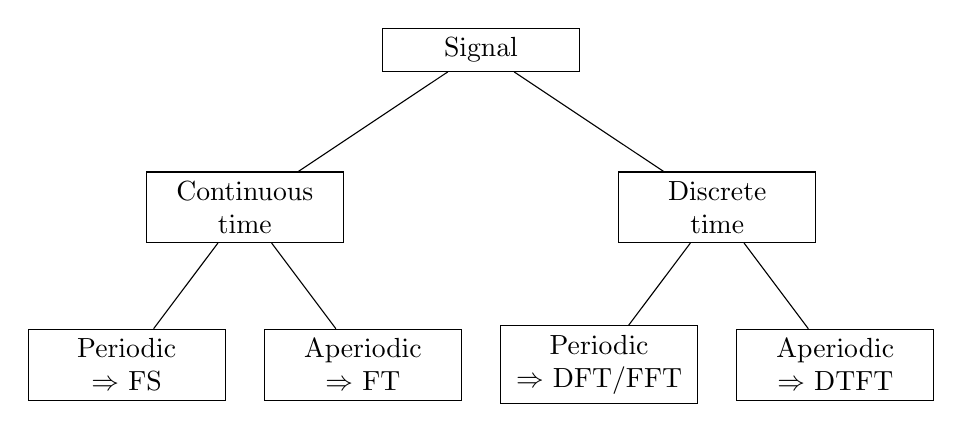
\begin{tikzpicture}[
  level 1/.style={sibling distance=6cm, level distance=2cm},
  level 2/.style={sibling distance=3cm, level distance=2cm},
  every node/.style={rectangle, draw, align=center, minimum width=2.5cm}
]

\node {Signal}
  child {node {Continuous\\ time}
    child {node {Periodic\\ $\Rightarrow$ FS}}
    child {node {Aperiodic\\ $\Rightarrow$ FT}}
  }
  child {node {Discrete\\ time}
    child {node {Periodic\\ $\Rightarrow$ DFT/FFT}}
    child {node {Aperiodic\\ $\Rightarrow$ DTFT}}
  };
\end{tikzpicture}
\end{center}

\subsection{Comparison Table}

\begin{center}
\small
\begin{tabular}{|l|c|c|c|c|}
\hline
\textbf{Transform} & \textbf{Time} & \textbf{Frequency} & \textbf{Forward} & \textbf{Inverse} \\
\hline
Fourier & Cont., & Discrete, & $c_n = \frac{1}{T}\int_0^T f(t) e^{-i2\pi nt/T} dt$ & $f(t) = \sum_n c_n e^{i2\pi nt/T}$ \\
Series (FS) & Periodic & Aperiodic & & \\
\hline
Fourier & Cont., & Cont., & $\hat{f}(\omega) = \int f(t) e^{-i\omega t} dt$ & $f(t) = \frac{1}{2\pi}\int \hat{f}(\omega) e^{i\omega t} d\omega$ \\
Transform (FT) & Aperiodic & Aperiodic & & \\
\hline
DTFT & Discrete, & Cont., & $X(e^{i\omega}) = \sum_n x[n] e^{-i\omega n}$ & $x[n] = \frac{1}{2\pi}\int_{-\pi}^{\pi} X(e^{i\omega}) e^{i\omega n} d\omega$ \\
& Aperiodic & Periodic & & \\
\hline
DFT & Discrete, & Discrete, & $X[k] = \sum_{n=0}^{N-1} x[n] e^{-i2\pi kn/N}$ & $x[n] = \frac{1}{N}\sum_{k=0}^{N-1} X[k] e^{i2\pi kn/N}$ \\
& Periodic & Periodic & & \\
\hline
FFT & \multicolumn{4}{c|}{Efficient algorithm for computing DFT in $O(N \log N)$ time} \\
\hline
\end{tabular}
\end{center}

\subsection{Conditions for Existence and Convergence}

\begin{center}
\begin{tabular}{|l|p{10cm}|}
\hline
\textbf{FS} & $f \in L^2([0,T])$ for $L^2$ convergence; Dirichlet conditions for pointwise convergence \\
\hline
\textbf{FT} & $f \in L^1(\R)$ for existence; $f \in L^2(\R)$ for Plancherel; additional smoothness for pointwise convergence \\
\hline
\textbf{DTFT} & $\sum_n \abs{x[n]} < \infty$ (absolutely summable sequences) \\
\hline
\textbf{DFT} & Always exists for finite sequences \\
\hline
\end{tabular}
\end{center}

\section{Applications and Examples}

\subsection{Solving Differential Equations}

\begin{example}[Heat Equation]
Consider the heat equation on $\R$:
\[
\frac{\partial u}{\partial t} = \alpha \frac{\partial^2 u}{\partial x^2}, \quad u(x, 0) = f(x).
\]

Apply the Fourier transform in $x$:
\[
\frac{\partial \hat{u}}{\partial t} = -\alpha \omega^2 \hat{u}.
\]

This is an ODE with solution:
\[
\hat{u}(\omega, t) = \hat{f}(\omega) e^{-\alpha \omega^2 t}.
\]

Inverse transform:
\[
u(x, t) = \frac{1}{2\pi} \int \hat{f}(\omega) e^{-\alpha \omega^2 t} e^{i\omega x} d\omega = (f * G_t)(x),
\]
where $G_t(x) = \frac{1}{\sqrt{4\pi \alpha t}} e^{-x^2/(4\alpha t)}$ is the heat kernel.
\end{example}

\subsection{Signal Processing}

\begin{example}[Ideal Low-Pass Filter]
An ideal low-pass filter has frequency response:
\[
H(\omega) = \begin{cases}
1 & \abs{\omega} < \omega_c \\
0 & \abs{\omega} > \omega_c
\end{cases}
\]

The impulse response is:
\[
h(t) = \frac{1}{2\pi} \int_{-\omega_c}^{\omega_c} e^{i\omega t} d\omega = \frac{\omega_c}{\pi} \sinc(\omega_c t/\pi).
\]

Note that $h(t)$ is non-causal and extends to $\pm \infty$, making it unrealizable in practice.
\end{example}

\subsection{Fast Convolution}

For long sequences, computing convolution directly takes $O(N^2)$ time. Using the FFT:
\begin{enumerate}
\item Zero-pad $x$ and $h$ to length $N \geq N_x + N_h - 1$.
\item Compute $X = \text{FFT}(x)$ and $H = \text{FFT}(h)$.
\item Compute $Y = X \cdot H$ (elementwise).
\item Compute $y = \text{IFFT}(Y)$.
\end{enumerate}

Total complexity: $O(N \log N)$.

\section{Advanced Topics}

\subsection{Windowing and Spectral Leakage}

When applying the DFT to a finite segment of a signal, we implicitly multiply by a rectangular window, causing spectral leakage.

\begin{definition}[Window Functions]
Common windows include:
\begin{itemize}
\item \textbf{Rectangular}: $w[n] = 1$
\item \textbf{Hamming}: $w[n] = 0.54 - 0.46\cos(2\pi n/(N-1))$
\item \textbf{Hann}: $w[n] = 0.5(1 - \cos(2\pi n/(N-1)))$
\item \textbf{Blackman}: $w[n] = 0.42 - 0.5\cos(2\pi n/(N-1)) + 0.08\cos(4\pi n/(N-1))$
\end{itemize}
\end{definition}

Windows trade off main-lobe width (frequency resolution) against side-lobe level (leakage).

\subsection{Short-Time Fourier Transform (STFT)}

For non-stationary signals, the STFT provides time-frequency localization:
\[
\text{STFT}_x(\tau, \omega) = \int x(t) w(t - \tau) e^{-i\omega t} dt,
\]
where $w(t)$ is a window function.

\subsection{Discrete Cosine Transform (DCT)}

The DCT is widely used in image and audio compression (JPEG, MP3):
\[
X[k] = \sum_{n=0}^{N-1} x[n] \cos\left(\frac{\pi k(2n+1)}{2N}\right).
\]

The DCT is real-valued and has excellent energy compaction properties for natural signals.

\subsection{Multidimensional Transforms}

The DFT extends naturally to higher dimensions:
\[
X[k_1, k_2] = \sum_{n_1=0}^{N_1-1} \sum_{n_2=0}^{N_2-1} x[n_1, n_2] e^{-i2\pi(k_1 n_1/N_1 + k_2 n_2/N_2)}.
\]

The 2D FFT is computed by applying 1D FFTs along each dimension (row-column algorithm).

\section{Conclusion}

The Fourier family of transforms provides a unified framework for frequency analysis:

\begin{itemize}
\item \textbf{Fourier Series}: Analyze periodic continuous-time signals
\item \textbf{Fourier Transform}: Analyze aperiodic continuous-time signals
\item \textbf{DTFT}: Analyze aperiodic discrete-time signals
\item \textbf{DFT}: Analyze periodic (or finite-length) discrete-time signals
\item \textbf{FFT}: Efficiently compute the DFT
\end{itemize}

Understanding the relationships between these transforms and the conditions under which each applies is essential for both theoretical analysis and practical applications in signal processing, communications, and computational science.

\chapterappendix

\section{Proofs of Advanced Theorems}

\subsection{Proof of Plancherel Theorem}

\begin{proof}
We prove this for $f \in L^1(\R) \cap L^2(\R)$, then extend by density.

Define the truncated functions $f_R(t) = f(t) \chi_{[-R,R]}(t)$. By the inversion formula:
\[
f_R(t) = \frac{1}{2\pi} \int \hat{f}_R(\omega) e^{i\omega t} d\omega.
\]

Multiply by $\overline{f(t)}$ and integrate:
\begin{align*}
\int f_R(t) \overline{f(t)} dt &= \frac{1}{2\pi} \int \left( \int \hat{f}_R(\omega) e^{i\omega t} d\omega \right) \overline{f(t)} dt \\
&= \frac{1}{2\pi} \int \hat{f}_R(\omega) \left( \int f(t) e^{-i\omega t} dt \right) d\omega \\
&= \frac{1}{2\pi} \int \hat{f}_R(\omega) \overline{\hat{f}(\omega)} d\omega.
\end{align*}

As $R \to \infty$, the left side converges to $\norm{f}_2^2$ and the right side to $\frac{1}{2\pi} \norm{\hat{f}}_2^2$ by dominated convergence.
\end{proof}

\subsection{Proof of Shannon Sampling Theorem}

\begin{proof}
Since $f$ is bandlimited, $\hat{f}(\omega) = 0$ for $\abs{\omega} > \omega_{\max}$. Extend $\hat{f}$ periodically with period $\omega_s > 2\omega_{\max}$:
\[
\hat{f}_p(\omega) = \sum_{k=-\infty}^{\infty} \hat{f}(\omega - k\omega_s).
\]

Since $\omega_s > 2\omega_{\max}$, there is no overlap and $\hat{f}_p(\omega) = \hat{f}(\omega)$ for $\abs{\omega} < \omega_s/2$.

The Fourier series coefficients of $\hat{f}_p$ are:
\[
c_n = \frac{1}{\omega_s} \int_{-\omega_s/2}^{\omega_s/2} \hat{f}(\omega) e^{i\omega n T_s} d\omega = \frac{1}{\omega_s} \int \hat{f}(\omega) e^{i\omega n T_s} d\omega = \frac{2\pi}{\omega_s} f(nT_s).
\]

Therefore:
\[
\hat{f}(\omega) = \hat{f}_p(\omega) = \sum_n c_n e^{-i\omega n T_s} = \frac{2\pi}{\omega_s} \sum_n f(nT_s) e^{-i\omega n T_s}.
\]

Inverse Fourier transform:
\[
f(t) = \frac{1}{2\pi} \int \hat{f}(\omega) e^{i\omega t} d\omega = \sum_n f(nT_s) \frac{1}{\omega_s} \int_{-\omega_s/2}^{\omega_s/2} e^{i\omega(t - nT_s)} d\omega.
\]

The integral evaluates to:
\[
\frac{1}{\omega_s} \int_{-\omega_s/2}^{\omega_s/2} e^{i\omega(t - nT_s)} d\omega = \frac{\sin(\omega_s(t - nT_s)/2)}{\omega_s(t - nT_s)/2} = T_s \sinc\left(\frac{t - nT_s}{T_s}\right).
\]
\end{proof}

\section{Exercises}

\begin{enumerate}
\item Compute the Fourier series of the sawtooth wave $f(t) = t$ for $-\pi < t < \pi$, extended periodically.

\item Show that the Fourier transform of $f(t) = e^{-a\abs{t}}$ for $a > 0$ is $\hat{f}(\omega) = \frac{2a}{a^2 + \omega^2}$.

\item Prove that if $f$ is even, $\hat{f}$ is real, and if $f$ is odd, $\hat{f}$ is purely imaginary.

\item Implement the radix-2 decimation-in-time FFT algorithm and verify it matches the DFT on random input.

\item Show that circular convolution becomes linear convolution when the sequences are zero-padded appropriately.

\item Compute the DTFT of the unit step sequence $u[n] = \begin{cases} 1 & n \geq 0 \\ 0 & n < 0 \end{cases}$ (carefully handle convergence).

\item Derive the relationship between the DFT and samples of the DTFT.

\item Analyze the effect of different window functions on spectral leakage using a pure sinusoid.
\end{enumerate}

\section{References}

\begin{enumerate}
\item Rudin, W. \emph{Real and Complex Analysis}. McGraw-Hill, 1987.
\item Oppenheim, A. V., and Schafer, R. W. \emph{Discrete-Time Signal Processing}. Pearson, 2009.
\item Stein, E. M., and Shakarchi, R. \emph{Fourier Analysis: An Introduction}. Princeton University Press, 2003.
\item Bracewell, R. N. \emph{The Fourier Transform and Its Applications}. McGraw-Hill, 2000.
\item Cooley, J. W., and Tukey, J. W. "An Algorithm for the Machine Calculation of Complex Fourier Series." \emph{Mathematics of Computation}, 1965.
\end{enumerate}
\end{notechapter}
